\section{Experiments}\label{sec:exp}
In this section, we conduct two sets of experiments. In the first part, we provide empirical support for our optimality theory in Section~\ref{sec:confidence} by evaluating the local likelihood optimization objective \eqref{eq:trainable_confidence} attained by different unmasking strategies in synthetic and real text generation tasks. In the second part, we train unmasking policies with \alg{} and evaluate the resulting sampling performance on text, code, and math benchmarks across multiple masked diffusion models (MDMs). In addition to the main comparisons with uniform and confidence-based unmasking, we also study the effect of KL regularization, temperature, and the per-step unmasking schedule.

\subsection{Numerical Analysis on Likelihood Optimization}

\begin{figure}[h]
    \centering
    \begin{subfigure}[h]{0.4\linewidth}
        \centering
        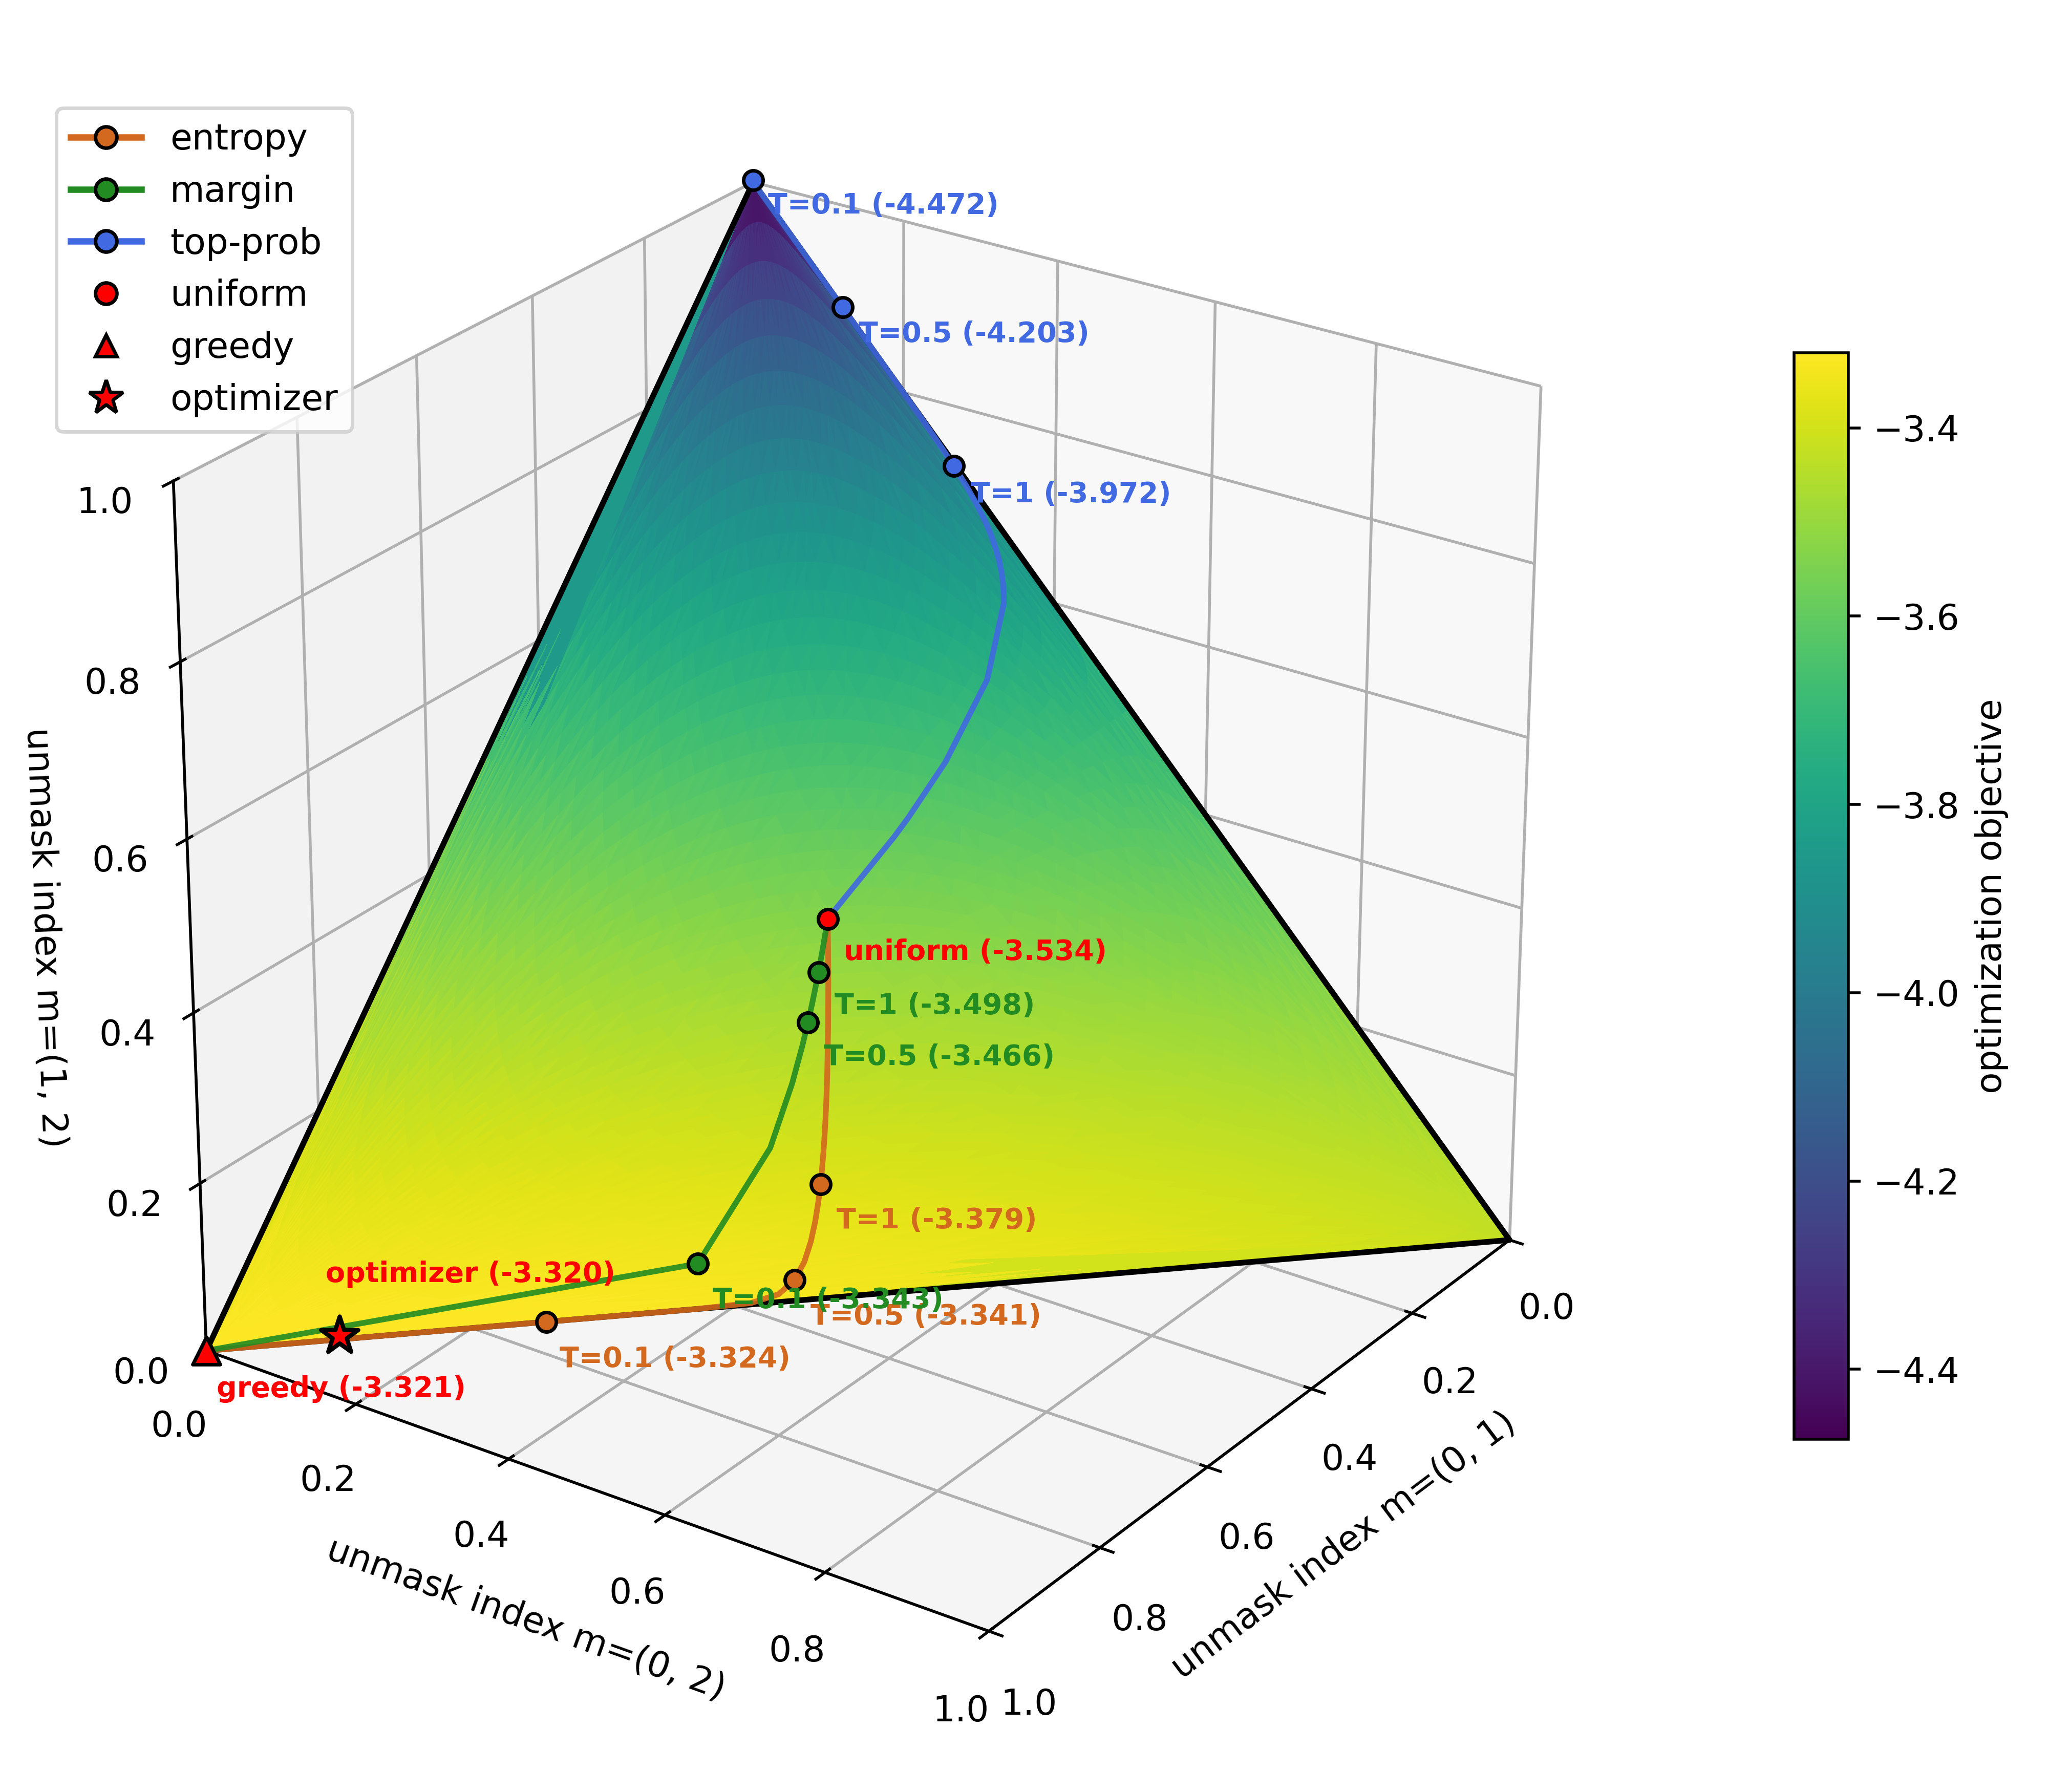
\includegraphics[width=\linewidth]{figs/policy_simplex.png}
        \vspace{-5pt}
        \caption{Landscape on the policy simplex.}
        \label{fig:opt-intro}
    \end{subfigure}
    \hfill
    \begin{subfigure}[h]{0.58\linewidth}
        \centering
        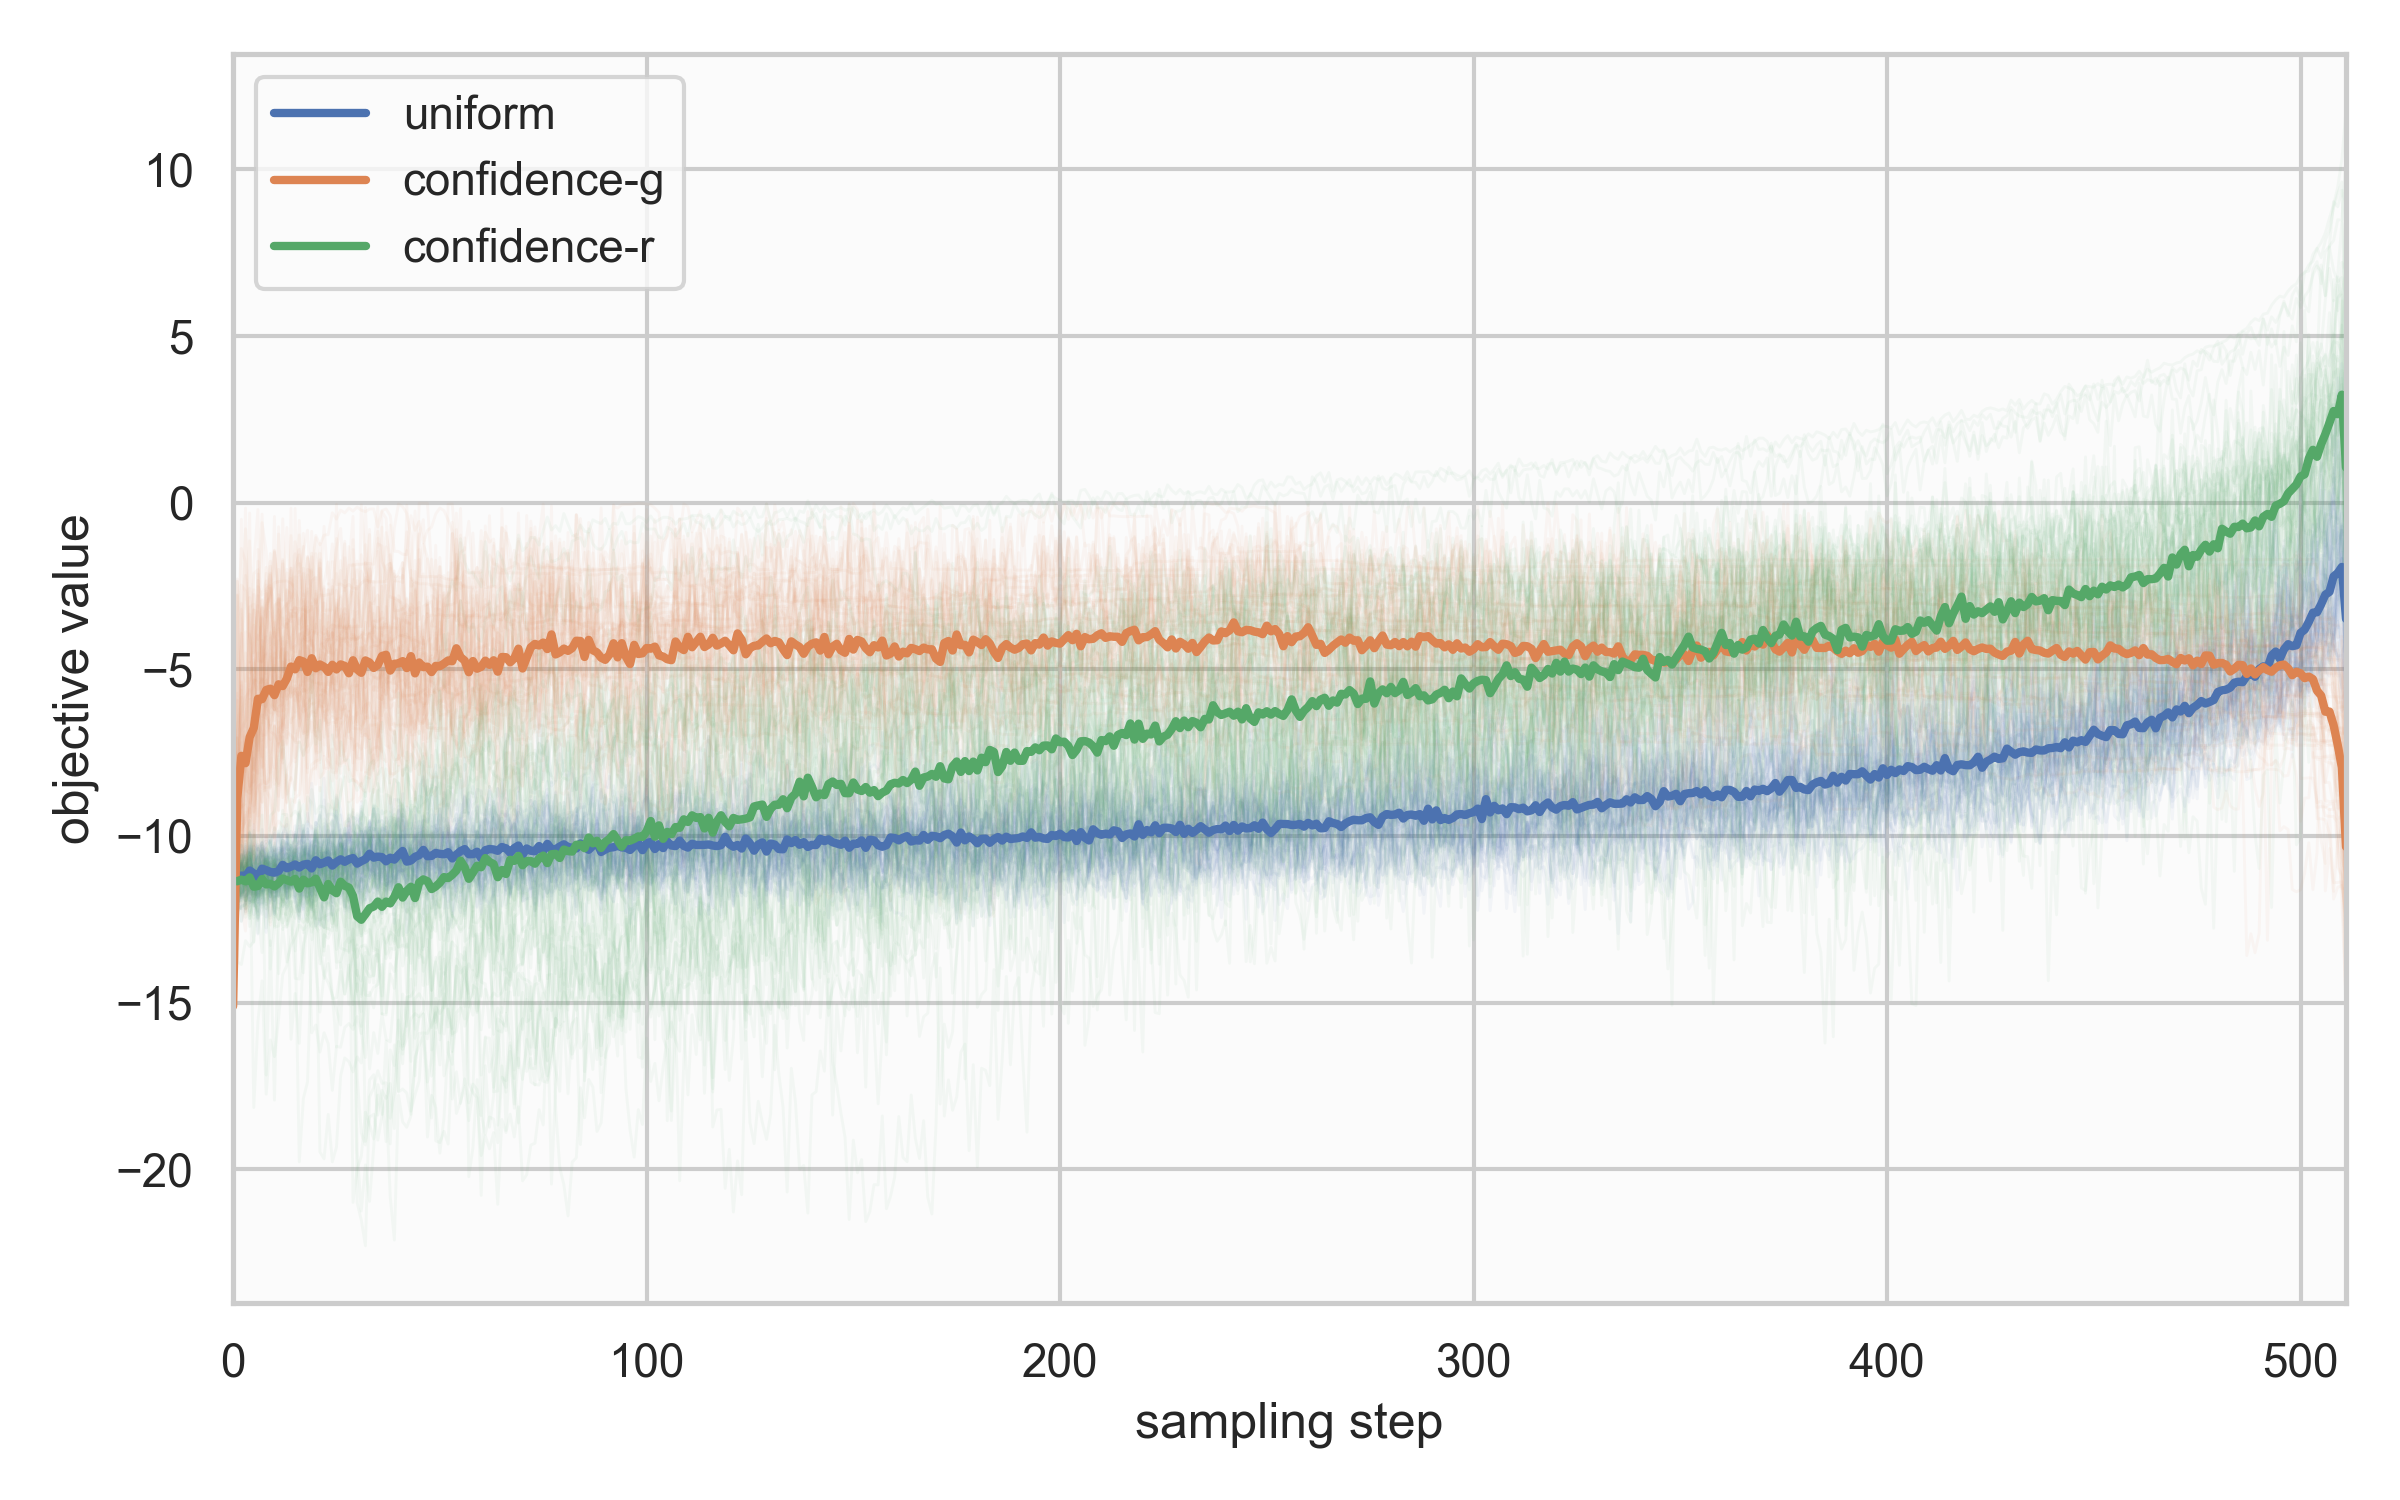
\includegraphics[width=\linewidth]{figs/objective_steps_512.png}
        \caption{Per-step objective values attained by unmasking strategies.}
        \label{fig:radd-obj-val}
    \end{subfigure}
    \label{fig:optimality-exp}
    \caption{Likelihood optimality analysis of unmasking strategies. \textbf{(a)}: The landscape of the local likelihood maximization problem \eqref{eq:trainable_confidence} over the policy simplex, under the synthetic task of unmasking 2 tokens from a length-3 sequence. We also plot different unmasking methods in the simplex and report their attained objective values. \textbf{(b)}: Monte Carlo estimation of local objective values \eqref{eq:trainable_confidence} attained by different unmasking methods in each step of 512-step text generation with RADD~\citep{ou2025absorbingdiscretediffusionsecretly}.}
\end{figure}

\paragraph{Landscape Visualization under Synthetic Distribution.}

We consider a task of unmasking 2 tokens from a length-3 sequence. There are exactly three possible unmasking actions: unmasking indices $\{0,1\}$, $\{0,2\}$, or $\{1,2\}$, enabling a full visualization of the optimization landscape in 3-dimensional space. To simulate MDM predictions $p_t^\theta(\cdot \mid \bm x_t)$, we use a synthetic distribution; see details in Appendix~\ref{subsec:synthetic}. In Figure~\ref{fig:opt-intro}, we plot the landscape and each unmasking method on the policy simplex. The exact optimizer of \eqref{eq:trainable_confidence} ($\bigstar$) is close to the entropy-based greedy point ($\blacktriangle$) with highly matching objective values, demonstrating Theorem~\ref{thm:confidence} and Theorem~\ref{thm:confidence-rand}. We provide additional results in Appendix~\ref{subsec:synthetic}. 

\paragraph{Objective Values in Real Text Generation.} 

We also evaluate the local objective value \eqref{eq:trainable_confidence} attained by different unmasking strategies in text generation using RADD~\citep{ou2024your}, a pretrained MDM. We compare uniform unmasking, greedy confidence unmasking based on the top-2 probability margin, and the randomized version. At each step, the objective \eqref{eq:trainable_confidence} is approximated by Monte Carlo estimation; see Appendix~\ref{subsec:radd-gen-exp}. In Figure~\ref{fig:radd-obj-val}, we set generation length to be 1024 and consider 512 diffusion sampling steps. We observe that both confidence methods consistently achieve higher objective values than the uniform method, in consistency with our theory in Section~\ref{sec:confidence}. See Appendix~\ref{subsec:radd-gen-exp} for further results.

\subsection{Evaluation of VLP}

\subsubsection{Text Generation}


\begin{wraptable}{r}{0.55\textwidth}
\caption{Average perplexity ($\downarrow$) of unconditional generations from RADD under different unmasking strategies and numbers of sampling steps. All generations have context length 1024.}
\centering
\small
\begin{tabular}{cccccc}
\toprule
steps & 16 & 32 & 64 & 128 & 256 \\
\midrule
uniform
& 335.1
& 199.7
& 154.5
& 132.2
& 118.9 \\
confidence-g
& 836.3
& 800.0
& 618.5
& 782.0
& 644.3 \\
confidence-r
& 308.7
& 186.3
& 132.4
& \textbf{109.2}
& \textbf{103.4} \\
\midrule
\cellcolor{lightblue}\alg{}
& \cellcolor{bestgreen}\textbf{293.2}
& \cellcolor{bestgreen}\textbf{179.6}
& \cellcolor{bestgreen}\textbf{130.3}
& \cellcolor{lightblue}116.9
& \cellcolor{lightblue}106.7 \\
\bottomrule
\end{tabular}
\label{tab:text-gen}
\end{wraptable}

For text generation, we evaluate \alg{} on RADD~\citep{ou2025absorbingdiscretediffusionsecretly}, a pretrained MDM for unconditional text generation. We train the unmasking policy on OpenWebText and evaluate generation quality using GPT-2 perplexity over sampling budgets from 16 to 256 steps. We compare against uniform unmasking and confidence unmasking based on top-2 probability margin, including both greedy and randomized variants. The detailed training and evaluation setup is provided in Appendix~\ref{sec:code-math-details}.

We report the GPT-2 perplexity of generated samples in Tables~\ref{tab:text-gen}. \alg{} substantially improves over uniform unmasking and matches or outperforms confidence-based methods, with the largest gains in the low-step regime. Randomized confidence unmasking is consistently stronger than greedy confidence unmasking, suggesting that deterministic high-confidence selection can be suboptimal.

\iffalse
\subsubsection{Code and Math Generation with DiffuCoder}
For code generation, we train our policy with DiffuCoder-7B-Instruct \citep{gong2025diffucoderunderstandingimprovingmasked}, a 7B-parameter MDM with strong coding performance after supervised fine-tuning on OpenCoder-SFT. The architecture of the policy network follows Section~\ref{subsec:architecture} and is approximately 1.5\% of the size of DiffuCoder. The policy is trained on the same SFT dataset. We reformat each query-output pair according to the chat template in Table~\ref{tab:chat-sft}, Appendix~\ref{sec:experiment-appendix}, following \citet{gong2025diffucoderunderstandingimprovingmasked}, and pad each chat to fixed length 1024 using DiffuCoder's padding token \texttt{<|dlm\_pad|>}. Following standard SFT practice for MDMs \citep{ye2025dream7bdiffusionlarge,nie2025largelanguagediffusionmodels,gong2025diffucoderunderstandingimprovingmasked}, we keep the prompt section intact during the masking and unmasking processes. We choose $K=16$ sampling steps, learning rate $\eta=0.001$, and $\lambda=0.1$ with AdamW optimizer.

We evaluate code generation using Pass@1 ($\uparrow$) on HumanEval \citep{chen2021evaluatinglargelanguagemodels} and MBPP \citep{austin2021programsynthesislargelanguage}. The evaluation chat templates are provided in Appendix~\ref{sec:experiment-appendix}. Results are reported in Table~\ref{tab:code-gen-diffucoder}. As in text generation, \alg{} consistently improves over uniform unmasking and outperforms confidence-based methods in most settings. Greedy confidence unmasking again performs poorly.

To examine whether the learned policy generalizes beyond coding, we additionally evaluate zero-shot math performance on GSM8K and MATH500 using the same DiffuCoder policy. Results are reported in Table~\ref{tab:math-diffucoder}. Since DiffuCoder is supervised-finetuned primarily on coding data, its absolute performance on math tasks is limited. Nevertheless, VLP remains competitive with or better than confidence-based unmasking at small and moderate step counts, indicating that the learned unmasking policy can transfer across domains.




\subsubsection{Broader Evaluation on Dream}
To better assess the behavior of the learned policy on models with stronger math ability, we additionally evaluate our method on Dream-7B \citep{ye2025dream7bdiffusionlarge}. Table~\ref{tab:dream-code} reports coding results on HumanEval and MBPP, while Table~\ref{tab:dream-math} reports math results on GSM8K and MATH500.

On coding benchmarks, the same trend holds: the learned policy improves over the model's original sampling strategy and generally outperforms confidence-based unmasking. On math benchmarks, VLP matches or surpasses confidence unmasking in most settings. These results strengthen the claim that VLP is not limited to DiffuCoder or coding-only tasks, but can transfer across models and domains.



\begin{table*}[h]
\centering
\caption{Results ($\uparrow$) of Dream-7B under different unmasking strategies and numbers of sampling steps across four benchmarks.}
\setlength{\tabcolsep}{4.5pt}
\resizebox{\textwidth}{!}{%
\begin{tabular}{ccccccccccccccccc}
\toprule
& \multicolumn{4}{c}{HumanEval} 
& \multicolumn{4}{c}{MBPP}
& \multicolumn{4}{c}{GSM8K}
& \multicolumn{4}{c}{MATH500} \\
\cmidrule(lr){2-5}\cmidrule(lr){6-9}\cmidrule(lr){10-13}\cmidrule(lr){14-17}
steps
& 16 & 32 & 64 & 128
& 16 & 32 & 64 & 128
& 16 & 32 & 64 & 128
& 16 & 32 & 64 & 128 \\
\midrule
uniform
& 8.5 & 17.6 & 19.5 & 23.2
& 18.6 & 25.6 & 27.6 & 30.8
& 23.4 & 30.0 & 34.9 & 35.4
& 10.4 & 12.8 & 13.8 & 16.8 \\
confidence-g
& 3.0 & 5.5 & 14.0 & 20.7
& 1.4 & 1.6 & 6.4 & 13.6
& 12.8 & 29.4 & \textbf{42.1} & \textbf{40.7}
& 3.6 & 7.0 & 15.0 & 12.0 \\
confidence-r
& 15.2 & 18.3 & 26.2 & 27.4
& \textbf{25.2} & 24.4 & 27.4 & 32.0
& 32.7 & 36.5 & 39.2 & 39.6
& 15.2 & 16.8 & 16.6 & 18.2 \\
\midrule
\cellcolor{lightblue}VLP
& \cellcolor{bestgreen}\textbf{17.0} & \cellcolor{bestgreen}\textbf{22.6} & \cellcolor{bestgreen}\textbf{27.4} & \cellcolor{bestgreen}\textbf{29.3}
& \cellcolor{lightblue}22.8 & \cellcolor{bestgreen}\textbf{26.2} & \cellcolor{bestgreen}\textbf{31.6} & \cellcolor{bestgreen}\textbf{32.8}
& \cellcolor{bestgreen}\textbf{33.6} & \cellcolor{bestgreen}\textbf{36.6} & \cellcolor{lightblue}38.3 & \cellcolor{lightblue}38.2
& \cellcolor{bestgreen}\textbf{15.6} & \cellcolor{bestgreen}\textbf{17.0} & \cellcolor{bestgreen}\textbf{17.2} & \cellcolor{bestgreen}\textbf{19.4} \\
\bottomrule
\end{tabular}%
}
\label{tab:dream-all}
\end{table*}

\fi


\subsubsection{Code and Math Generation}

We evaluate \alg{} on code and math generation using two 7B-scale MDMs: Dream-7B~\citep{ye2025dream7bdiffusionlarge} and DiffuCoder-7B~\citep{gong2025diffucoderunderstandingimprovingmasked}. We train the policy with OpenCoder-SFT and MetaMathQA dataset, and evaluate on two code generation benchmarks: HumanEval~\citep{chen2021evaluatinglargelanguagemodels} as well as MBPP~\citep{austin2021programsynthesislargelanguage}, and two math generation benchmarks: GSM8K~\citep{?} and MATH500~\citep{?}. The detailed setup is provided in Appendix~\ref{sec:vlp}.

Results on both models are summarized in Tables~\ref{tab:dream-all} and~\ref{tab:diffucoder-all} (deferred to Appendix~\ref{sec:vlp-additional-results}). Across Dream and DiffuCoder, \alg{} consistently matches or outperforms confidence-based unmasking, especially at small and moderate sampling budgets. Both \alg{} and random confidence method display a clear improvement from the vanilla uniform unmasking. Greedy confidence unmasking often performs poorly, suggesting that deterministic confidence selection can be suboptimal. These results indicate that likelihood-trained unmasking policies can provide robust gains across various models, sampling budgets, and task domains.

\begin{table*}[h]
\centering
\caption{Results ($\uparrow$) of Dream-7B under different unmasking strategies and numbers of sampling steps across four benchmarks.}
\setlength{\tabcolsep}{4.5pt}
\resizebox{\textwidth}{!}{%
\begin{tabular}{ccccccccccccccccc}
\toprule
& \multicolumn{4}{c}{HumanEval} 
& \multicolumn{4}{c}{MBPP}
& \multicolumn{4}{c}{GSM8K}
& \multicolumn{4}{c}{MATH500} \\
\cmidrule(lr){2-5}\cmidrule(lr){6-9}\cmidrule(lr){10-13}\cmidrule(lr){14-17}
steps
& 16 & 32 & 64 & 128
& 16 & 32 & 64 & 128
& 16 & 32 & 64 & 128
& 16 & 32 & 64 & 128 \\
\midrule
uniform
& 8.5 & 17.6 & 19.5 & 23.2
& 18.6 & 25.6 & 27.6 & 30.8
& 23.4 & 30.0 & 34.9 & 35.4
& 10.4 & 12.8 & 13.8 & 16.8 \\
confidence-g
& 3.0 & 5.5 & 14.0 & 20.7
& 1.4 & 1.6 & 6.4 & 13.6
& 12.8 & 29.4 & \textbf{42.1} & \textbf{40.7}
& 3.6 & 7.0 & 15.0 & 12.0 \\
confidence-r
& 15.2 & 18.3 & 26.2 & 27.4
& \textbf{25.2} & 24.4 & 27.4 & 32.0
& 32.7 & 36.5 & 39.2 & 39.6
& 15.2 & 16.8 & 16.6 & 18.2 \\
\midrule
\cellcolor{lightblue}VLP
& \cellcolor{bestgreen}\textbf{17.0} & \cellcolor{bestgreen}\textbf{22.6} & \cellcolor{bestgreen}\textbf{27.4} & \cellcolor{bestgreen}\textbf{29.3}
& \cellcolor{lightblue}22.8 & \cellcolor{bestgreen}\textbf{26.2} & \cellcolor{bestgreen}\textbf{31.6} & \cellcolor{bestgreen}\textbf{32.8}
& \cellcolor{bestgreen}\textbf{33.6} & \cellcolor{bestgreen}\textbf{36.6} & \cellcolor{lightblue}38.3 & \cellcolor{lightblue}38.2
& \cellcolor{bestgreen}\textbf{15.6} & \cellcolor{bestgreen}\textbf{17.0} & \cellcolor{bestgreen}\textbf{17.2} & \cellcolor{bestgreen}\textbf{19.4} \\
\bottomrule
\end{tabular}%
}
\label{tab:dream-all}
\end{table*}

\subsubsection{Ablation Studies}

\paragraph{Effect of KL regularization.}

\paragraph{Choice of $K$ in training.}
